\problemname{Mars Message}

I the film \emph{The Martian}, astronaut Mark Watney is stuck on Mars, and communicates with earth by rotating a camera on an old space prod.

The prod points ar a hexidecimal digit, i.e. \texttt{0-9} or \texttt{a-f}, and Mark creates letters and other characters by konverting a pair
of hexadecimal digits accordning to ASCII encoding. The determine which digit the pond is pointing at Mark has divided a circle of 360 degrees into 16 parts of 22.5 degrees each.

\begin{figure}[h!]
  \begin{center}
    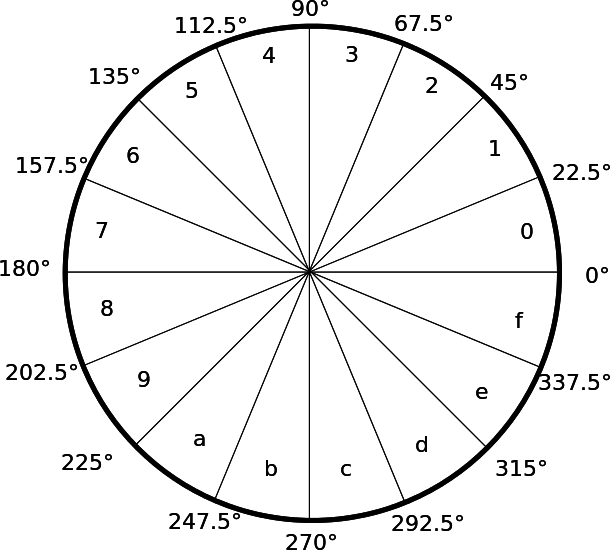
\includegraphics[width=0.4\textwidth]{angles.png}
  \end{center}
\end{figure}

For example, the pair of angles $(100*{\circ}, 30^{\circ})$ represents the hexadecimal number \texttt{0x41}, which in decimal is $65$.
According to ASCII that is the character \texttt{A}.

Mark is getting tired of writing down the digits manually, and he asks you to help him decode the messages he receives. You will be given the sequence of angles the prod points at and you're expected to print the message.

\section*{Input}
The first line consists of an integer $2 \le N \le 50\,000$, the number of angles. $N$ will be even.

The following $N$ lines contain angles, one angle per line. An angle is given in degrees as a float in the range $[0, 360)$

De nästa $N$ raderna innehåller vinklarna, en vinkel per rad. Vinkeln ges som ett flyttal i grader i intervallet $[0, 360)$.
Det är garanterat att sonden aldrig pekar på någon vinkel som två hexadecimala siffror har gemensamt.

Det är också garanterat att under avkodningen till ASCII kommer enbart tecken med decimala värden \texttt{32-126} ges.

\section*{Output}
Du ska skriva ut en enda rad med de tecken som meddelandet avkodas till.

\section*{Poängsättning}
Din lösning kommer att testas på en mängd testfallsgrupper. För att få poäng för en grupp så måste du klara alla testfall i gruppen.

\begin{tabular}{| l | l | l |}
	\hline
	Grupp & Poängvärde & Begränsningar\\ \hline
  1     & 46         & alla vinklar är heltal \\ \hline
  2     & 54         & \\ \hline
\end{tabular}
